\documentclass[1p]{elsarticle_modified}
%\bibliographystyle{elsarticle-num}

%\usepackage[colorlinks]{hyperref}
%\usepackage{abbrmath_seonhwa} %\Abb, \Ascr, \Acal ,\Abf, \Afrak
\usepackage{amsfonts}
\usepackage{amssymb}
\usepackage{amsmath}
\usepackage{amsthm}
\usepackage{scalefnt}
\usepackage{amsbsy}
\usepackage{kotex}
\usepackage{caption}
\usepackage{subfig}
\usepackage{color}
\usepackage{graphicx}
\usepackage{xcolor} %% white, black, red, green, blue, cyan, magenta, yellow
\usepackage{float}
\usepackage{setspace}
\usepackage{hyperref}

\usepackage{tikz}
\usetikzlibrary{arrows}

\usepackage{multirow}
\usepackage{array} % fixed length table
\usepackage{hhline}

%%%%%%%%%%%%%%%%%%%%%
\makeatletter
\renewcommand*\env@matrix[1][\arraystretch]{%
	\edef\arraystretch{#1}%
	\hskip -\arraycolsep
	\let\@ifnextchar\new@ifnextchar
	\array{*\c@MaxMatrixCols c}}
\makeatother %https://tex.stackexchange.com/questions/14071/how-can-i-increase-the-line-spacing-in-a-matrix
%%%%%%%%%%%%%%%

\usepackage[normalem]{ulem}

\newcommand{\msout}[1]{\ifmmode\text{\sout{\ensuremath{#1}}}\else\sout{#1}\fi}
%SOURCE: \msout is \stkout macro in https://tex.stackexchange.com/questions/20609/strikeout-in-math-mode

\newcommand{\cancel}[1]{
	\ifmmode
	{\color{red}\msout{#1}}
	\else
	{\color{red}\sout{#1}}
	\fi
}

\newcommand{\add}[1]{
	{\color{blue}\uwave{#1}}
}

\newcommand{\replace}[2]{
	\ifmmode
	{\color{red}\msout{#1}}{\color{blue}\uwave{#2}}
	\else
	{\color{red}\sout{#1}}{\color{blue}\uwave{#2}}
	\fi
}

\newcommand{\Sol}{\mathcal{S}} %segment
\newcommand{\D}{D} %diagram
\newcommand{\A}{\mathcal{A}} %arc


%%%%%%%%%%%%%%%%%%%%%%%%%%%%%5 test

\def\sl{\operatorname{\textup{SL}}(2,\Cbb)}
\def\psl{\operatorname{\textup{PSL}}(2,\Cbb)}
\def\quan{\mkern 1mu \triangleright \mkern 1mu}

\theoremstyle{definition}
\newtheorem{thm}{Theorem}[section]
\newtheorem{prop}[thm]{Proposition}
\newtheorem{lem}[thm]{Lemma}
\newtheorem{ques}[thm]{Question}
\newtheorem{cor}[thm]{Corollary}
\newtheorem{defn}[thm]{Definition}
\newtheorem{exam}[thm]{Example}
\newtheorem{rmk}[thm]{Remark}
\newtheorem{alg}[thm]{Algorithm}

\newcommand{\I}{\sqrt{-1}}
\begin{document}

%\begin{frontmatter}
%
%\title{Boundary parabolic representations of knots up to 8 crossings}
%
%%% Group authors per affiliation:
%\author{Yunhi Cho} 
%\address{Department of Mathematics, University of Seoul, Seoul, Korea}
%\ead{yhcho@uos.ac.kr}
%
%
%\author{Seonhwa Kim} %\fnref{s_kim}}
%\address{Center for Geometry and Physics, Institute for Basic Science, Pohang, 37673, Korea}
%\ead{ryeona17@ibs.re.kr}
%
%\author{Hyuk Kim}
%\address{Department of Mathematical Sciences, Seoul National University, Seoul 08826, Korea}
%\ead{hyukkim@snu.ac.kr}
%
%\author{Seokbeom Yoon}
%\address{Department of Mathematical Sciences, Seoul National University, Seoul, 08826,  Korea}
%\ead{sbyoon15@snu.ac.kr}
%
%\begin{abstract}
%We find all boundary parabolic representation of knots up to 8 crossings.
%
%\end{abstract}
%\begin{keyword}
%    \MSC[2010] 57M25 
%\end{keyword}
%
%\end{frontmatter}

%\linenumbers
%\tableofcontents
%
\newcommand\colored[1]{\textcolor{white}{\rule[-0.35ex]{0.8em}{1.4ex}}\kern-0.8em\color{red} #1}%
%\newcommand\colored[1]{\textcolor{white}{ #1}\kern-2.17ex	\textcolor{white}{ #1}\kern-1.81ex	\textcolor{white}{ #1}\kern-2.15ex\color{red}#1	}

{\Large $\underline{12a_{1231}~(K12a_{1231})}$}

\setlength{\tabcolsep}{10pt}
\renewcommand{\arraystretch}{1.6}
\vspace{1cm}\begin{tabular}{m{100pt}>{\centering\arraybackslash}m{274pt}}
\multirow{5}{120pt}{
	\centering
	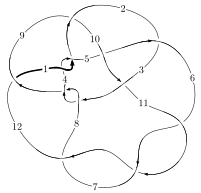
\includegraphics[width=112pt]{../../../GIT/diagram.site/Diagrams/png/2032_12a_1231.png}\\
\ \ \ A knot diagram\footnotemark}&
\allowdisplaybreaks
\textbf{Linearized knot diagam} \\
\cline{2-2}
 &
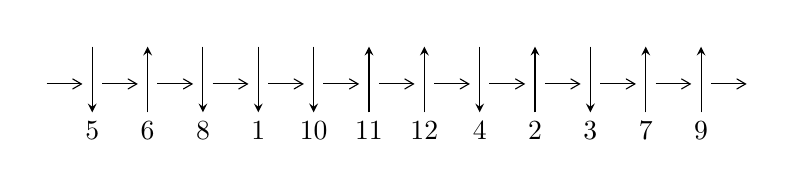
\begin{tikzpicture}[x=20pt, y=17pt]
	% nodes
	\node (C0) at (0, 0) {};
	\node (C1) at (1, 0) {};
	\node (C1U) at (1, +1) {};
	\node (C1D) at (1, -1) {5};

	\node (C2) at (2, 0) {};
	\node (C2U) at (2, +1) {};
	\node (C2D) at (2, -1) {6};

	\node (C3) at (3, 0) {};
	\node (C3U) at (3, +1) {};
	\node (C3D) at (3, -1) {8};

	\node (C4) at (4, 0) {};
	\node (C4U) at (4, +1) {};
	\node (C4D) at (4, -1) {1};

	\node (C5) at (5, 0) {};
	\node (C5U) at (5, +1) {};
	\node (C5D) at (5, -1) {10};

	\node (C6) at (6, 0) {};
	\node (C6U) at (6, +1) {};
	\node (C6D) at (6, -1) {11};

	\node (C7) at (7, 0) {};
	\node (C7U) at (7, +1) {};
	\node (C7D) at (7, -1) {12};

	\node (C8) at (8, 0) {};
	\node (C8U) at (8, +1) {};
	\node (C8D) at (8, -1) {4};

	\node (C9) at (9, 0) {};
	\node (C9U) at (9, +1) {};
	\node (C9D) at (9, -1) {2};

	\node (C10) at (10, 0) {};
	\node (C10U) at (10, +1) {};
	\node (C10D) at (10, -1) {3};

	\node (C11) at (11, 0) {};
	\node (C11U) at (11, +1) {};
	\node (C11D) at (11, -1) {7};

	\node (C12) at (12, 0) {};
	\node (C12U) at (12, +1) {};
	\node (C12D) at (12, -1) {9};
	\node (C13) at (13, 0) {};

	% arrows
	\draw[->,>={angle 60}]
	(C0) edge (C1) (C1) edge (C2) (C2) edge (C3) (C3) edge (C4) (C4) edge (C5) (C5) edge (C6) (C6) edge (C7) (C7) edge (C8) (C8) edge (C9) (C9) edge (C10) (C10) edge (C11) (C11) edge (C12) (C12) edge (C13) ;	\draw[->,>=stealth]
	(C1U) edge (C1D) (C2D) edge (C2U) (C3U) edge (C3D) (C4U) edge (C4D) (C5U) edge (C5D) (C6D) edge (C6U) (C7D) edge (C7U) (C8U) edge (C8D) (C9D) edge (C9U) (C10U) edge (C10D) (C11D) edge (C11U) (C12D) edge (C12U) ;
	\end{tikzpicture} \\
\hhline{~~} \\& 
\textbf{Solving Sequence} \\ \cline{2-2} 
 &
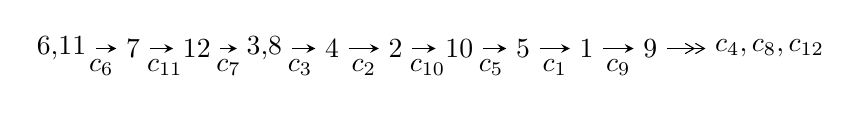
\begin{tikzpicture}[x=23pt, y=7pt]
	% node
	\node (A0) at (-1/8, 0) {6,11};
	\node (A1) at (1, 0) {7};
	\node (A2) at (2, 0) {12};
	\node (A3) at (49/16, 0) {3,8};
	\node (A4) at (33/8, 0) {4};
	\node (A5) at (41/8, 0) {2};
	\node (A6) at (49/8, 0) {10};
	\node (A7) at (57/8, 0) {5};
	\node (A8) at (65/8, 0) {1};
	\node (A9) at (73/8, 0) {9};
	\node (C1) at (1/2, -1) {$c_{6}$};
	\node (C2) at (3/2, -1) {$c_{11}$};
	\node (C3) at (5/2, -1) {$c_{7}$};
	\node (C4) at (29/8, -1) {$c_{3}$};
	\node (C5) at (37/8, -1) {$c_{2}$};
	\node (C6) at (45/8, -1) {$c_{10}$};
	\node (C7) at (53/8, -1) {$c_{5}$};
	\node (C8) at (61/8, -1) {$c_{1}$};
	\node (C9) at (69/8, -1) {$c_{9}$};
	\node (A10) at (11, 0) {$c_{4},c_{8},c_{12}$};

	% edge
	\draw[->,>=stealth]	
	(A0) edge (A1) (A1) edge (A2) (A2) edge (A3) (A3) edge (A4) (A4) edge (A5) (A5) edge (A6) (A6) edge (A7) (A7) edge (A8) (A8) edge (A9) ;
	\draw[->>,>={angle 60}]	
	(A9) edge (A10);
\end{tikzpicture} \\ 

\end{tabular} \\

\footnotetext{
The image of knot diagram is generated by the software ``\textbf{Draw programme}" developed by Andrew Bartholomew(\url{http://www.layer8.co.uk/maths/draw/index.htm\#Running-draw}), where we modified some parts for our purpose(\url{https://github.com/CATsTAILs/LinksPainter}).
}\phantom \\ \newline 
\centering \textbf{Ideals for irreducible components\footnotemark of $X_{\text{par}}$} 
 
\begin{align*}
I^u_{1}&=\langle 
1.99754\times10^{289} u^{111}+1.22647\times10^{289} u^{110}+\cdots+2.03815\times10^{287} b-6.40655\times10^{289},\\
\phantom{I^u_{1}}&\phantom{= \langle  }1.12492\times10^{290} u^{111}+8.47128\times10^{289} u^{110}+\cdots+2.03815\times10^{287} a-2.42251\times10^{290},\\
\phantom{I^u_{1}}&\phantom{= \langle  }2 u^{112}+u^{111}+\cdots-30 u+1\rangle \\
I^u_{2}&=\langle 
-32 u^{15}-74 u^{14}+\cdots+43 b+23,\;-40 u^{15}-28 u^{14}+\cdots+43 a-68,\;2 u^{16}+3 u^{15}+\cdots+2 u+1\rangle \\
\\
\end{align*}
\raggedright * 2 irreducible components of $\dim_{\mathbb{C}}=0$, with total 128 representations.\\
\footnotetext{All coefficients of polynomials are rational numbers. But the coefficients are sometimes approximated in decimal forms when there is not enough margin.}
\newpage
\renewcommand{\arraystretch}{1}
\centering \section*{I. $I^u_{1}= \langle 2.00\times10^{289} u^{111}+1.23\times10^{289} u^{110}+\cdots+2.04\times10^{287} b-6.41\times10^{289},\;1.12\times10^{290} u^{111}+8.47\times10^{289} u^{110}+\cdots+2.04\times10^{287} a-2.42\times10^{290},\;2 u^{112}+u^{111}+\cdots-30 u+1 \rangle$}
\flushleft \textbf{(i) Arc colorings}\\
\begin{tabular}{m{7pt} m{180pt} m{7pt} m{180pt} }
\flushright $a_{6}=$&$\begin{pmatrix}1\\0\end{pmatrix}$ \\
\flushright $a_{11}=$&$\begin{pmatrix}0\\u\end{pmatrix}$ \\
\flushright $a_{7}=$&$\begin{pmatrix}1\\- u^2\end{pmatrix}$ \\
\flushright $a_{12}=$&$\begin{pmatrix}u\\- u^3+u\end{pmatrix}$ \\
\flushright $a_{3}=$&$\begin{pmatrix}-551.935 u^{111}-415.637 u^{110}+\cdots-29550.2 u+1188.58\\-98.0077 u^{111}-60.1758 u^{110}+\cdots-7598.38 u+314.332\end{pmatrix}$ \\
\flushright $a_{8}=$&$\begin{pmatrix}- u^2+1\\u^4-2 u^2\end{pmatrix}$ \\
\flushright $a_{4}=$&$\begin{pmatrix}-394.383 u^{111}-312.399 u^{110}+\cdots-18944.3 u+760.560\\-105.829 u^{111}-65.1082 u^{110}+\cdots-8246.34 u+341.293\end{pmatrix}$ \\
\flushright $a_{2}=$&$\begin{pmatrix}-453.928 u^{111}-355.461 u^{110}+\cdots-21951.8 u+874.251\\-98.0077 u^{111}-60.1758 u^{110}+\cdots-7598.38 u+314.332\end{pmatrix}$ \\
\flushright $a_{10}=$&$\begin{pmatrix}908.353 u^{111}+637.752 u^{110}+\cdots+52318.5 u-2021.35\\30.7684 u^{111}+20.7117 u^{110}+\cdots+2266.98 u-91.6692\end{pmatrix}$ \\
\flushright $a_{5}=$&$\begin{pmatrix}-1139.83 u^{111}-842.942 u^{110}+\cdots-59872.7 u+2318.75\\-92.0889 u^{111}-59.4474 u^{110}+\cdots-6446.70 u+256.944\end{pmatrix}$ \\
\flushright $a_{1}=$&$\begin{pmatrix}1108.35 u^{111}+819.201 u^{110}+\cdots+58304.1 u-2258.52\\99.3976 u^{111}+64.4297 u^{110}+\cdots+7036.59 u-281.533\end{pmatrix}$ \\
\flushright $a_{9}=$&$\begin{pmatrix}552.407 u^{111}+373.353 u^{110}+\cdots+35614.1 u-1396.31\\-38.5186 u^{111}-24.3200 u^{110}+\cdots-3107.36 u+134.687\end{pmatrix}$\\&\end{tabular}
\flushleft \textbf{(ii) Obstruction class $= -1$}\\~\\
\flushleft \textbf{(iii) Cusp Shapes $= 353.645 u^{111}+195.115 u^{110}+\cdots+38493.2 u-1748.36$}\\~\\
\newpage\renewcommand{\arraystretch}{1}
\flushleft \textbf{(iv) u-Polynomials at the component}\newline \\
\begin{tabular}{m{50pt}|m{274pt}}
Crossings & \hspace{64pt}u-Polynomials at each crossing \\
\hline $$\begin{aligned}c_{1},c_{4}\end{aligned}$$&$\begin{aligned}
&2(2 u^{112}-3 u^{111}+\cdots+6 u-1)
\end{aligned}$\\
\hline $$\begin{aligned}c_{2}\end{aligned}$$&$\begin{aligned}
&u^{112}+u^{111}+\cdots+33183 u+20078
\end{aligned}$\\
\hline $$\begin{aligned}c_{3},c_{8}\end{aligned}$$&$\begin{aligned}
&u^{112}-4 u^{111}+\cdots-18821 u-1439
\end{aligned}$\\
\hline $$\begin{aligned}c_{5}\end{aligned}$$&$\begin{aligned}
&2(2 u^{112}-5 u^{111}+\cdots+1262 u-211)
\end{aligned}$\\
\hline $$\begin{aligned}c_{6},c_{7},c_{11}\end{aligned}$$&$\begin{aligned}
&2(2 u^{112}- u^{111}+\cdots+30 u+1)
\end{aligned}$\\
\hline $$\begin{aligned}c_{9}\end{aligned}$$&$\begin{aligned}
&u^{112}-5 u^{110}+\cdots-17 u+1
\end{aligned}$\\
\hline $$\begin{aligned}c_{10}\end{aligned}$$&$\begin{aligned}
&u^{112}-3 u^{111}+\cdots+1445 u+116
\end{aligned}$\\
\hline $$\begin{aligned}c_{12}\end{aligned}$$&$\begin{aligned}
&u^{112}-3 u^{111}+\cdots+4391 u-2366
\end{aligned}$\\
\hline
\end{tabular}\\~\\
\newpage\renewcommand{\arraystretch}{1}
\flushleft \textbf{(v) Riley Polynomials at the component}\newline \\
\begin{tabular}{m{50pt}|m{274pt}}
Crossings & \hspace{64pt}Riley Polynomials at each crossing \\
\hline $$\begin{aligned}c_{1},c_{4}\end{aligned}$$&$\begin{aligned}
&4(4 y^{112}-365 y^{111}+\cdots-942 y+1)
\end{aligned}$\\
\hline $$\begin{aligned}c_{2}\end{aligned}$$&$\begin{aligned}
&y^{112}-51 y^{111}+\cdots-21359572553 y+403126084
\end{aligned}$\\
\hline $$\begin{aligned}c_{3},c_{8}\end{aligned}$$&$\begin{aligned}
&y^{112}-92 y^{111}+\cdots-91920487 y+2070721
\end{aligned}$\\
\hline $$\begin{aligned}c_{5}\end{aligned}$$&$\begin{aligned}
&4(4 y^{112}-121 y^{111}+\cdots-1692236 y+44521)
\end{aligned}$\\
\hline $$\begin{aligned}c_{6},c_{7},c_{11}\end{aligned}$$&$\begin{aligned}
&4(4 y^{112}-457 y^{111}+\cdots-108 y+1)
\end{aligned}$\\
\hline $$\begin{aligned}c_{9}\end{aligned}$$&$\begin{aligned}
&y^{112}-10 y^{111}+\cdots-1271 y+1
\end{aligned}$\\
\hline $$\begin{aligned}c_{10}\end{aligned}$$&$\begin{aligned}
&y^{112}+9 y^{111}+\cdots-1322657 y+13456
\end{aligned}$\\
\hline $$\begin{aligned}c_{12}\end{aligned}$$&$\begin{aligned}
&y^{112}+21 y^{111}+\cdots+215563547 y+5597956
\end{aligned}$\\
\hline
\end{tabular}\\~\\
\newpage\flushleft \textbf{(vi) Complex Volumes and Cusp Shapes}
$$\begin{array}{c|c|c}  
\text{Solutions to }I^u_{1}& \I (\text{vol} + \sqrt{-1}CS) & \text{Cusp shape}\\
 \hline 
\begin{aligned}
u &= -0.590366 + 0.885349 I \\
a &= -0.102462 + 1.298050 I \\
b &= -1.11216 + 0.87568 I\end{aligned}
 & -6.8356 - 13.8442 I & \phantom{-0.000000 } 0 \\ \hline\begin{aligned}
u &= -0.590366 - 0.885349 I \\
a &= -0.102462 - 1.298050 I \\
b &= -1.11216 - 0.87568 I\end{aligned}
 & -6.8356 + 13.8442 I & \phantom{-0.000000 } 0 \\ \hline\begin{aligned}
u &= \phantom{-}0.387376 + 0.820027 I \\
a &= \phantom{-}0.801976 + 0.900426 I \\
b &= \phantom{-}0.781284 + 0.066752 I\end{aligned}
 & -3.17183 + 5.58573 I & \phantom{-0.000000 } 0 \\ \hline\begin{aligned}
u &= \phantom{-}0.387376 - 0.820027 I \\
a &= \phantom{-}0.801976 - 0.900426 I \\
b &= \phantom{-}0.781284 - 0.066752 I\end{aligned}
 & -3.17183 - 5.58573 I & \phantom{-0.000000 } 0 \\ \hline\begin{aligned}
u &= -0.950565 + 0.582823 I \\
a &= \phantom{-}0.885922 + 0.749010 I \\
b &= -1.100390 + 0.730571 I\end{aligned}
 & -6.07516 + 1.98826 I & \phantom{-0.000000 } 0 \\ \hline\begin{aligned}
u &= -0.950565 - 0.582823 I \\
a &= \phantom{-}0.885922 - 0.749010 I \\
b &= -1.100390 - 0.730571 I\end{aligned}
 & -6.07516 - 1.98826 I & \phantom{-0.000000 } 0 \\ \hline\begin{aligned}
u &= -0.539116 + 0.977111 I \\
a &= \phantom{-}0.196917 - 1.010420 I \\
b &= \phantom{-}1.002550 - 0.842221 I\end{aligned}
 & -0.90925 - 8.02423 I & \phantom{-0.000000 } 0 \\ \hline\begin{aligned}
u &= -0.539116 - 0.977111 I \\
a &= \phantom{-}0.196917 + 1.010420 I \\
b &= \phantom{-}1.002550 + 0.842221 I\end{aligned}
 & -0.90925 + 8.02423 I & \phantom{-0.000000 } 0 \\ \hline\begin{aligned}
u &= \phantom{-}1.092700 + 0.292344 I \\
a &= \phantom{-}0.299720 + 0.356342 I \\
b &= \phantom{-}0.547701 + 0.773817 I\end{aligned}
 & -1.53248 - 1.05574 I & \phantom{-0.000000 } 0 \\ \hline\begin{aligned}
u &= \phantom{-}1.092700 - 0.292344 I \\
a &= \phantom{-}0.299720 - 0.356342 I \\
b &= \phantom{-}0.547701 - 0.773817 I\end{aligned}
 & -1.53248 + 1.05574 I & \phantom{-0.000000 } 0\\
 \hline 
 \end{array}$$\newpage$$\begin{array}{c|c|c}  
\text{Solutions to }I^u_{1}& \I (\text{vol} + \sqrt{-1}CS) & \text{Cusp shape}\\
 \hline 
\begin{aligned}
u &= -0.569748 + 1.005160 I \\
a &= -0.600229 - 0.292334 I \\
b &= -0.782709 - 0.777145 I\end{aligned}
 & -6.96272 + 7.75772 I & \phantom{-0.000000 } 0 \\ \hline\begin{aligned}
u &= -0.569748 - 1.005160 I \\
a &= -0.600229 + 0.292334 I \\
b &= -0.782709 + 0.777145 I\end{aligned}
 & -6.96272 - 7.75772 I & \phantom{-0.000000 } 0 \\ \hline\begin{aligned}
u &= \phantom{-}0.508841 + 0.643434 I \\
a &= \phantom{-}0.24252 - 1.69762 I \\
b &= -0.517859 - 0.894564 I\end{aligned}
 & -7.91872 + 5.18418 I & \phantom{-0.000000 } 0 \\ \hline\begin{aligned}
u &= \phantom{-}0.508841 - 0.643434 I \\
a &= \phantom{-}0.24252 + 1.69762 I \\
b &= -0.517859 + 0.894564 I\end{aligned}
 & -7.91872 - 5.18418 I & \phantom{-0.000000 } 0 \\ \hline\begin{aligned}
u &= -1.091250 + 0.502566 I \\
a &= \phantom{-}0.295839 - 0.306431 I \\
b &= \phantom{-}0.629753 + 0.307422 I\end{aligned}
 & \phantom{-}0.932453 + 0.972249 I & \phantom{-0.000000 } 0 \\ \hline\begin{aligned}
u &= -1.091250 - 0.502566 I \\
a &= \phantom{-}0.295839 + 0.306431 I \\
b &= \phantom{-}0.629753 - 0.307422 I\end{aligned}
 & \phantom{-}0.932453 - 0.972249 I & \phantom{-0.000000 } 0 \\ \hline\begin{aligned}
u &= \phantom{-}0.761966 + 0.237108 I \\
a &= -1.217380 + 0.027406 I \\
b &= -1.100330 + 0.223061 I\end{aligned}
 & -5.06841 - 0.08229 I & \phantom{-0.000000 } 0 \\ \hline\begin{aligned}
u &= \phantom{-}0.761966 - 0.237108 I \\
a &= -1.217380 - 0.027406 I \\
b &= -1.100330 - 0.223061 I\end{aligned}
 & -5.06841 + 0.08229 I & \phantom{-0.000000 } 0 \\ \hline\begin{aligned}
u &= -0.233694 + 0.757943 I \\
a &= -0.310289 - 1.045990 I \\
b &= -0.679733 - 1.177870 I\end{aligned}
 & -8.18021 - 6.63313 I & \phantom{-0.000000 } 0 \\ \hline\begin{aligned}
u &= -0.233694 - 0.757943 I \\
a &= -0.310289 + 1.045990 I \\
b &= -0.679733 + 1.177870 I\end{aligned}
 & -8.18021 + 6.63313 I & \phantom{-0.000000 } 0\\
 \hline 
 \end{array}$$\newpage$$\begin{array}{c|c|c}  
\text{Solutions to }I^u_{1}& \I (\text{vol} + \sqrt{-1}CS) & \text{Cusp shape}\\
 \hline 
\begin{aligned}
u &= \phantom{-}0.439423 + 0.650359 I \\
a &= \phantom{-}0.15580 + 1.70235 I \\
b &= \phantom{-}0.736097 + 0.616610 I\end{aligned}
 & -3.30092 + 3.97805 I & \phantom{-0.000000 } 0 \\ \hline\begin{aligned}
u &= \phantom{-}0.439423 - 0.650359 I \\
a &= \phantom{-}0.15580 - 1.70235 I \\
b &= \phantom{-}0.736097 - 0.616610 I\end{aligned}
 & -3.30092 - 3.97805 I & \phantom{-0.000000 } 0 \\ \hline\begin{aligned}
u &= -0.534981 + 0.567137 I \\
a &= -0.582903 + 0.852307 I \\
b &= -0.771986 + 0.127212 I\end{aligned}
 & \phantom{-}0.65467 - 1.94051 I & \phantom{-0.000000 } 0 \\ \hline\begin{aligned}
u &= -0.534981 - 0.567137 I \\
a &= -0.582903 - 0.852307 I \\
b &= -0.771986 - 0.127212 I\end{aligned}
 & \phantom{-}0.65467 + 1.94051 I & \phantom{-0.000000 } 0 \\ \hline\begin{aligned}
u &= \phantom{-}0.561224 + 0.521086 I \\
a &= \phantom{-}0.04561 + 1.65702 I \\
b &= \phantom{-}1.077830 + 0.903388 I\end{aligned}
 & -1.78856 + 8.81527 I & \phantom{-0.000000 } 0 \\ \hline\begin{aligned}
u &= \phantom{-}0.561224 - 0.521086 I \\
a &= \phantom{-}0.04561 - 1.65702 I \\
b &= \phantom{-}1.077830 - 0.903388 I\end{aligned}
 & -1.78856 - 8.81527 I & \phantom{-0.000000 } 0 \\ \hline\begin{aligned}
u &= \phantom{-}0.476725 + 0.579061 I \\
a &= -1.06705 + 0.99583 I \\
b &= -0.390123 + 0.719749 I\end{aligned}
 & -7.95289 - 0.98790 I & \phantom{-0.000000 } 0 \\ \hline\begin{aligned}
u &= \phantom{-}0.476725 - 0.579061 I \\
a &= -1.06705 - 0.99583 I \\
b &= -0.390123 - 0.719749 I\end{aligned}
 & -7.95289 + 0.98790 I & \phantom{-0.000000 } 0 \\ \hline\begin{aligned}
u &= -0.744686 + 0.010412 I \\
a &= -0.900370 + 0.365272 I \\
b &= \phantom{-}0.523275 - 0.136180 I\end{aligned}
 & \phantom{-}1.62810 - 0.09506 I & \phantom{-0.000000 } 0 \\ \hline\begin{aligned}
u &= -0.744686 - 0.010412 I \\
a &= -0.900370 - 0.365272 I \\
b &= \phantom{-}0.523275 + 0.136180 I\end{aligned}
 & \phantom{-}1.62810 + 0.09506 I & \phantom{-0.000000 } 0\\
 \hline 
 \end{array}$$\newpage$$\begin{array}{c|c|c}  
\text{Solutions to }I^u_{1}& \I (\text{vol} + \sqrt{-1}CS) & \text{Cusp shape}\\
 \hline 
\begin{aligned}
u &= \phantom{-}0.558961 + 0.469651 I \\
a &= \phantom{-}0.086448 - 1.405570 I \\
b &= -1.112160 - 0.800844 I\end{aligned}
 & \phantom{-}2.12676 + 4.19302 I & \phantom{-0.000000 } 0 \\ \hline\begin{aligned}
u &= \phantom{-}0.558961 - 0.469651 I \\
a &= \phantom{-}0.086448 + 1.405570 I \\
b &= -1.112160 + 0.800844 I\end{aligned}
 & \phantom{-}2.12676 - 4.19302 I & \phantom{-0.000000 } 0 \\ \hline\begin{aligned}
u &= \phantom{-}0.333560 + 0.645536 I \\
a &= -0.60141 - 2.16439 I \\
b &= -0.966813 - 0.578879 I\end{aligned}
 & -6.44067 + 3.62679 I & \phantom{-0.000000 } 0 \\ \hline\begin{aligned}
u &= \phantom{-}0.333560 - 0.645536 I \\
a &= -0.60141 + 2.16439 I \\
b &= -0.966813 + 0.578879 I\end{aligned}
 & -6.44067 - 3.62679 I & \phantom{-0.000000 } 0 \\ \hline\begin{aligned}
u &= \phantom{-}0.183486 + 0.680996 I \\
a &= -0.199275 + 0.770862 I \\
b &= \phantom{-}0.707467 + 1.002360 I\end{aligned}
 & -1.70178 - 1.37820 I & \phantom{-0.000000 } 0 \\ \hline\begin{aligned}
u &= \phantom{-}0.183486 - 0.680996 I \\
a &= -0.199275 - 0.770862 I \\
b &= \phantom{-}0.707467 - 1.002360 I\end{aligned}
 & -1.70178 + 1.37820 I & \phantom{-0.000000 } 0 \\ \hline\begin{aligned}
u &= \phantom{-}0.613446 + 0.336149 I \\
a &= \phantom{-}1.071940 - 0.252155 I \\
b &= \phantom{-}0.733101 - 0.271972 I\end{aligned}
 & -2.67908 - 0.14330 I & \phantom{-0.000000 } 0 \\ \hline\begin{aligned}
u &= \phantom{-}0.613446 - 0.336149 I \\
a &= \phantom{-}1.071940 + 0.252155 I \\
b &= \phantom{-}0.733101 + 0.271972 I\end{aligned}
 & -2.67908 + 0.14330 I & \phantom{-0.000000 } 0 \\ \hline\begin{aligned}
u &= \phantom{-}0.160538 + 0.675799 I \\
a &= \phantom{-}1.37339 - 0.67453 I \\
b &= \phantom{-}0.822486 - 0.666790 I\end{aligned}
 & -3.00254 - 5.11079 I & \phantom{-0.000000 } 0 \\ \hline\begin{aligned}
u &= \phantom{-}0.160538 - 0.675799 I \\
a &= \phantom{-}1.37339 + 0.67453 I \\
b &= \phantom{-}0.822486 + 0.666790 I\end{aligned}
 & -3.00254 + 5.11079 I & \phantom{-0.000000 } 0\\
 \hline 
 \end{array}$$\newpage$$\begin{array}{c|c|c}  
\text{Solutions to }I^u_{1}& \I (\text{vol} + \sqrt{-1}CS) & \text{Cusp shape}\\
 \hline 
\begin{aligned}
u &= \phantom{-}1.298430 + 0.235302 I \\
a &= \phantom{-}0.102389 - 0.314641 I \\
b &= -0.08777 - 1.51926 I\end{aligned}
 & \phantom{-}1.96152 + 4.82767 I & \phantom{-0.000000 } 0 \\ \hline\begin{aligned}
u &= \phantom{-}1.298430 - 0.235302 I \\
a &= \phantom{-}0.102389 + 0.314641 I \\
b &= -0.08777 + 1.51926 I\end{aligned}
 & \phantom{-}1.96152 - 4.82767 I & \phantom{-0.000000 } 0 \\ \hline\begin{aligned}
u &= \phantom{-}1.343260 + 0.024703 I \\
a &= -0.79980 + 1.39977 I \\
b &= \phantom{-}1.038890 + 0.659096 I\end{aligned}
 & -0.12150 + 6.44986 I & \phantom{-0.000000 } 0 \\ \hline\begin{aligned}
u &= \phantom{-}1.343260 - 0.024703 I \\
a &= -0.79980 - 1.39977 I \\
b &= \phantom{-}1.038890 - 0.659096 I\end{aligned}
 & -0.12150 - 6.44986 I & \phantom{-0.000000 } 0 \\ \hline\begin{aligned}
u &= \phantom{-}1.366240 + 0.046024 I \\
a &= \phantom{-}0.560578 - 0.987074 I \\
b &= -1.091950 - 0.866032 I\end{aligned}
 & \phantom{-}4.33941 + 2.95088 I & \phantom{-0.000000 } 0 \\ \hline\begin{aligned}
u &= \phantom{-}1.366240 - 0.046024 I \\
a &= \phantom{-}0.560578 + 0.987074 I \\
b &= -1.091950 + 0.866032 I\end{aligned}
 & \phantom{-}4.33941 - 2.95088 I & \phantom{-0.000000 } 0 \\ \hline\begin{aligned}
u &= \phantom{-}1.36756\phantom{ +0.000000I} \\
a &= \phantom{-}1.72809\phantom{ +0.000000I} \\
b &= -1.32458\phantom{ +0.000000I}\end{aligned}
 & -3.87440\phantom{ +0.000000I} & \phantom{-0.000000 } 0 \\ \hline\begin{aligned}
u &= -1.375580 + 0.054428 I \\
a &= -0.058414 + 0.233208 I \\
b &= \phantom{-}0.85136 + 1.17842 I\end{aligned}
 & \phantom{-}2.73981 - 0.95287 I & \phantom{-0.000000 } 0 \\ \hline\begin{aligned}
u &= -1.375580 - 0.054428 I \\
a &= -0.058414 - 0.233208 I \\
b &= \phantom{-}0.85136 - 1.17842 I\end{aligned}
 & \phantom{-}2.73981 + 0.95287 I & \phantom{-0.000000 } 0 \\ \hline\begin{aligned}
u &= \phantom{-}1.39179\phantom{ +0.000000I} \\
a &= -0.665022\phantom{ +0.000000I} \\
b &= \phantom{-}2.65741\phantom{ +0.000000I}\end{aligned}
 & \phantom{-}2.05074\phantom{ +0.000000I} & \phantom{-0.000000 } 0\\
 \hline 
 \end{array}$$\newpage$$\begin{array}{c|c|c}  
\text{Solutions to }I^u_{1}& \I (\text{vol} + \sqrt{-1}CS) & \text{Cusp shape}\\
 \hline 
\begin{aligned}
u &= -1.391760 + 0.151237 I \\
a &= -0.346628 - 0.427342 I \\
b &= -0.538958 - 0.756680 I\end{aligned}
 & -2.05807 - 1.42124 I & \phantom{-0.000000 } 0 \\ \hline\begin{aligned}
u &= -1.391760 - 0.151237 I \\
a &= -0.346628 + 0.427342 I \\
b &= -0.538958 + 0.756680 I\end{aligned}
 & -2.05807 + 1.42124 I & \phantom{-0.000000 } 0 \\ \hline\begin{aligned}
u &= \phantom{-}1.383380 + 0.245331 I \\
a &= -0.200611 + 0.257569 I \\
b &= -0.27130 + 1.55987 I\end{aligned}
 & -3.06588 + 10.17870 I & \phantom{-0.000000 } 0 \\ \hline\begin{aligned}
u &= \phantom{-}1.383380 - 0.245331 I \\
a &= -0.200611 - 0.257569 I \\
b &= -0.27130 - 1.55987 I\end{aligned}
 & -3.06588 - 10.17870 I & \phantom{-0.000000 } 0 \\ \hline\begin{aligned}
u &= \phantom{-}1.405420 + 0.025980 I \\
a &= -0.354219 + 0.448139 I \\
b &= \phantom{-}1.72762 + 2.16535 I\end{aligned}
 & \phantom{-}1.99770 - 0.22845 I & \phantom{-0.000000 } 0 \\ \hline\begin{aligned}
u &= \phantom{-}1.405420 - 0.025980 I \\
a &= -0.354219 - 0.448139 I \\
b &= \phantom{-}1.72762 - 2.16535 I\end{aligned}
 & \phantom{-}1.99770 + 0.22845 I & \phantom{-0.000000 } 0 \\ \hline\begin{aligned}
u &= \phantom{-}0.465488 + 0.351819 I \\
a &= \phantom{-}0.023333 + 0.303003 I \\
b &= \phantom{-}0.930736 + 0.639447 I\end{aligned}
 & -1.84150 - 1.16696 I & \phantom{-0.000000 } 0 \\ \hline\begin{aligned}
u &= \phantom{-}0.465488 - 0.351819 I \\
a &= \phantom{-}0.023333 - 0.303003 I \\
b &= \phantom{-}0.930736 - 0.639447 I\end{aligned}
 & -1.84150 + 1.16696 I & \phantom{-0.000000 } 0 \\ \hline\begin{aligned}
u &= -1.42221 + 0.03410 I \\
a &= -0.842144 + 0.248954 I \\
b &= \phantom{-}1.123970 + 0.118692 I\end{aligned}
 & \phantom{-}3.31166 - 0.09381 I & \phantom{-0.000000 } 0 \\ \hline\begin{aligned}
u &= -1.42221 - 0.03410 I \\
a &= -0.842144 - 0.248954 I \\
b &= \phantom{-}1.123970 - 0.118692 I\end{aligned}
 & \phantom{-}3.31166 + 0.09381 I & \phantom{-0.000000 } 0\\
 \hline 
 \end{array}$$\newpage$$\begin{array}{c|c|c}  
\text{Solutions to }I^u_{1}& \I (\text{vol} + \sqrt{-1}CS) & \text{Cusp shape}\\
 \hline 
\begin{aligned}
u &= \phantom{-}0.30230 + 1.39371 I \\
a &= -0.297118 + 0.046754 I \\
b &= -0.387699 + 0.464785 I\end{aligned}
 & -0.486493 + 0.007462 I & \phantom{-0.000000 } 0 \\ \hline\begin{aligned}
u &= \phantom{-}0.30230 - 1.39371 I \\
a &= -0.297118 - 0.046754 I \\
b &= -0.387699 - 0.464785 I\end{aligned}
 & -0.486493 - 0.007462 I & \phantom{-0.000000 } 0 \\ \hline\begin{aligned}
u &= -1.43585 + 0.06329 I \\
a &= \phantom{-}0.832002 - 0.993622 I \\
b &= -0.807707 - 0.181747 I\end{aligned}
 & \phantom{-}6.17126 - 3.60997 I & \phantom{-0.000000 } 0 \\ \hline\begin{aligned}
u &= -1.43585 - 0.06329 I \\
a &= \phantom{-}0.832002 + 0.993622 I \\
b &= -0.807707 + 0.181747 I\end{aligned}
 & \phantom{-}6.17126 + 3.60997 I & \phantom{-0.000000 } 0 \\ \hline\begin{aligned}
u &= -1.43996\phantom{ +0.000000I} \\
a &= \phantom{-}0.0590229\phantom{ +0.000000I} \\
b &= -3.67297\phantom{ +0.000000I}\end{aligned}
 & \phantom{-}1.33127\phantom{ +0.000000I} & \phantom{-0.000000 } 0 \\ \hline\begin{aligned}
u &= -1.44182 + 0.06731 I \\
a &= -0.63195 + 1.46857 I \\
b &= \phantom{-}0.664139 + 0.183670 I\end{aligned}
 & \phantom{-}1.59046 - 7.35618 I & \phantom{-0.000000 } 0 \\ \hline\begin{aligned}
u &= -1.44182 - 0.06731 I \\
a &= -0.63195 - 1.46857 I \\
b &= \phantom{-}0.664139 - 0.183670 I\end{aligned}
 & \phantom{-}1.59046 + 7.35618 I & \phantom{-0.000000 } 0 \\ \hline\begin{aligned}
u &= -0.149075 + 0.504192 I \\
a &= -0.94511 + 1.14088 I \\
b &= -0.610927 + 0.572174 I\end{aligned}
 & \phantom{-}0.054414 - 1.368480 I & \phantom{-}0.99794 + 3.85630 I \\ \hline\begin{aligned}
u &= -0.149075 - 0.504192 I \\
a &= -0.94511 - 1.14088 I \\
b &= -0.610927 - 0.572174 I\end{aligned}
 & \phantom{-}0.054414 + 1.368480 I & \phantom{-}0.99794 - 3.85630 I \\ \hline\begin{aligned}
u &= -1.46329 + 0.22171 I \\
a &= \phantom{-}0.72474 + 1.35578 I \\
b &= -1.044330 + 0.649176 I\end{aligned}
 & -0.58596 - 6.75157 I & \phantom{-0.000000 } 0\\
 \hline 
 \end{array}$$\newpage$$\begin{array}{c|c|c}  
\text{Solutions to }I^u_{1}& \I (\text{vol} + \sqrt{-1}CS) & \text{Cusp shape}\\
 \hline 
\begin{aligned}
u &= -1.46329 - 0.22171 I \\
a &= \phantom{-}0.72474 - 1.35578 I \\
b &= -1.044330 - 0.649176 I\end{aligned}
 & -0.58596 + 6.75157 I & \phantom{-0.000000 } 0 \\ \hline\begin{aligned}
u &= -0.510457 + 0.086922 I \\
a &= \phantom{-}1.97887 - 1.81247 I \\
b &= -0.265064 + 0.377912 I\end{aligned}
 & -1.94431 - 2.13405 I & \phantom{-}2.32412 + 6.81583 I \\ \hline\begin{aligned}
u &= -0.510457 - 0.086922 I \\
a &= \phantom{-}1.97887 + 1.81247 I \\
b &= -0.265064 - 0.377912 I\end{aligned}
 & -1.94431 + 2.13405 I & \phantom{-}2.32412 - 6.81583 I \\ \hline\begin{aligned}
u &= -1.50348 + 0.22309 I \\
a &= -0.638772 - 1.061640 I \\
b &= \phantom{-}0.928579 - 0.720640 I\end{aligned}
 & \phantom{-}3.07735 - 7.15990 I & \phantom{-0.000000 } 0 \\ \hline\begin{aligned}
u &= -1.50348 - 0.22309 I \\
a &= -0.638772 + 1.061640 I \\
b &= \phantom{-}0.928579 + 0.720640 I\end{aligned}
 & \phantom{-}3.07735 + 7.15990 I & \phantom{-0.000000 } 0 \\ \hline\begin{aligned}
u &= -1.49388 + 0.30393 I \\
a &= -0.125412 - 1.084930 I \\
b &= \phantom{-}0.983426 - 0.345192 I\end{aligned}
 & \phantom{-}2.93583 - 9.67376 I & \phantom{-0.000000 } 0 \\ \hline\begin{aligned}
u &= -1.49388 - 0.30393 I \\
a &= -0.125412 + 1.084930 I \\
b &= \phantom{-}0.983426 + 0.345192 I\end{aligned}
 & \phantom{-}2.93583 + 9.67376 I & \phantom{-0.000000 } 0 \\ \hline\begin{aligned}
u &= -1.51421 + 0.17868 I \\
a &= \phantom{-}0.666131 + 0.742857 I \\
b &= -1.49902 + 0.79847 I\end{aligned}
 & \phantom{-}8.91590 - 6.68730 I & \phantom{-0.000000 } 0 \\ \hline\begin{aligned}
u &= -1.51421 - 0.17868 I \\
a &= \phantom{-}0.666131 - 0.742857 I \\
b &= -1.49902 - 0.79847 I\end{aligned}
 & \phantom{-}8.91590 + 6.68730 I & \phantom{-0.000000 } 0 \\ \hline\begin{aligned}
u &= \phantom{-}1.46393 + 0.42707 I \\
a &= \phantom{-}0.400574 - 0.703058 I \\
b &= -1.32675 - 0.90235 I\end{aligned}
 & \phantom{-}4.14729 + 5.81797 I & \phantom{-0.000000 } 0\\
 \hline 
 \end{array}$$\newpage$$\begin{array}{c|c|c}  
\text{Solutions to }I^u_{1}& \I (\text{vol} + \sqrt{-1}CS) & \text{Cusp shape}\\
 \hline 
\begin{aligned}
u &= \phantom{-}1.46393 - 0.42707 I \\
a &= \phantom{-}0.400574 + 0.703058 I \\
b &= -1.32675 + 0.90235 I\end{aligned}
 & \phantom{-}4.14729 - 5.81797 I & \phantom{-0.000000 } 0 \\ \hline\begin{aligned}
u &= \phantom{-}1.51736 + 0.17092 I \\
a &= \phantom{-}0.279173 - 0.805873 I \\
b &= -1.032590 - 0.401616 I\end{aligned}
 & \phantom{-}7.44180 + 4.58976 I & \phantom{-0.000000 } 0 \\ \hline\begin{aligned}
u &= \phantom{-}1.51736 - 0.17092 I \\
a &= \phantom{-}0.279173 + 0.805873 I \\
b &= -1.032590 + 0.401616 I\end{aligned}
 & \phantom{-}7.44180 - 4.58976 I & \phantom{-0.000000 } 0 \\ \hline\begin{aligned}
u &= -1.51512 + 0.19650 I \\
a &= -0.719707 - 0.510490 I \\
b &= \phantom{-}1.55153 - 0.53896 I\end{aligned}
 & \phantom{-}4.63698 - 1.67249 I & \phantom{-0.000000 } 0 \\ \hline\begin{aligned}
u &= -1.51512 - 0.19650 I \\
a &= -0.719707 + 0.510490 I \\
b &= \phantom{-}1.55153 + 0.53896 I\end{aligned}
 & \phantom{-}4.63698 + 1.67249 I & \phantom{-0.000000 } 0 \\ \hline\begin{aligned}
u &= -1.51971 + 0.18217 I \\
a &= -0.643184 - 0.856014 I \\
b &= \phantom{-}1.42249 - 0.96880 I\end{aligned}
 & \phantom{-}5.03581 - 11.44180 I & \phantom{-0.000000 } 0 \\ \hline\begin{aligned}
u &= -1.51971 - 0.18217 I \\
a &= -0.643184 + 0.856014 I \\
b &= \phantom{-}1.42249 + 0.96880 I\end{aligned}
 & \phantom{-}5.03581 + 11.44180 I & \phantom{-0.000000 } 0 \\ \hline\begin{aligned}
u &= \phantom{-}0.385385 + 0.257518 I \\
a &= -1.69933 + 1.27300 I \\
b &= \phantom{-}0.979834 + 0.468293 I\end{aligned}
 & -2.59766 - 0.34195 I & -6.16678 - 7.93909 I \\ \hline\begin{aligned}
u &= \phantom{-}0.385385 - 0.257518 I \\
a &= -1.69933 - 1.27300 I \\
b &= \phantom{-}0.979834 - 0.468293 I\end{aligned}
 & -2.59766 + 0.34195 I & -6.16678 + 7.93909 I \\ \hline\begin{aligned}
u &= \phantom{-}1.53672 + 0.02430 I \\
a &= \phantom{-}0.854452 - 1.028970 I \\
b &= -0.518225 - 0.117988 I\end{aligned}
 & \phantom{-}4.99245 - 2.15881 I & \phantom{-0.000000 } 0\\
 \hline 
 \end{array}$$\newpage$$\begin{array}{c|c|c}  
\text{Solutions to }I^u_{1}& \I (\text{vol} + \sqrt{-1}CS) & \text{Cusp shape}\\
 \hline 
\begin{aligned}
u &= \phantom{-}1.53672 - 0.02430 I \\
a &= \phantom{-}0.854452 + 1.028970 I \\
b &= -0.518225 + 0.117988 I\end{aligned}
 & \phantom{-}4.99245 + 2.15881 I & \phantom{-0.000000 } 0 \\ \hline\begin{aligned}
u &= -1.52434 + 0.21328 I \\
a &= \phantom{-}0.684131 + 0.935220 I \\
b &= -0.722279 + 0.945973 I\end{aligned}
 & -1.23112 - 8.31311 I & \phantom{-0.000000 } 0 \\ \hline\begin{aligned}
u &= -1.52434 - 0.21328 I \\
a &= \phantom{-}0.684131 - 0.935220 I \\
b &= -0.722279 - 0.945973 I\end{aligned}
 & -1.23112 + 8.31311 I & \phantom{-0.000000 } 0 \\ \hline\begin{aligned}
u &= \phantom{-}1.57037 + 0.10518 I \\
a &= -0.464481 + 0.675080 I \\
b &= \phantom{-}0.830325 + 0.188200 I\end{aligned}
 & \phantom{-}9.68462 + 0.75111 I & \phantom{-0.000000 } 0 \\ \hline\begin{aligned}
u &= \phantom{-}1.57037 - 0.10518 I \\
a &= -0.464481 - 0.675080 I \\
b &= \phantom{-}0.830325 - 0.188200 I\end{aligned}
 & \phantom{-}9.68462 - 0.75111 I & \phantom{-0.000000 } 0 \\ \hline\begin{aligned}
u &= -1.54872 + 0.33463 I \\
a &= \phantom{-}0.120186 + 0.778443 I \\
b &= -0.794087 + 0.209483 I\end{aligned}
 & \phantom{-}6.13408 - 5.25289 I & \phantom{-0.000000 } 0 \\ \hline\begin{aligned}
u &= -1.54872 - 0.33463 I \\
a &= \phantom{-}0.120186 - 0.778443 I \\
b &= -0.794087 - 0.209483 I\end{aligned}
 & \phantom{-}6.13408 + 5.25289 I & \phantom{-0.000000 } 0 \\ \hline\begin{aligned}
u &= \phantom{-}1.54991 + 0.33692 I \\
a &= -0.560707 + 0.875963 I \\
b &= \phantom{-}1.36205 + 0.83316 I\end{aligned}
 & \phantom{-}5.82114 + 12.74530 I & \phantom{-0.000000 } 0 \\ \hline\begin{aligned}
u &= \phantom{-}1.54991 - 0.33692 I \\
a &= -0.560707 - 0.875963 I \\
b &= \phantom{-}1.36205 - 0.83316 I\end{aligned}
 & \phantom{-}5.82114 - 12.74530 I & \phantom{-0.000000 } 0 \\ \hline\begin{aligned}
u &= \phantom{-}1.56442 + 0.31341 I \\
a &= \phantom{-}0.658091 - 0.958017 I \\
b &= -1.35610 - 0.85602 I\end{aligned}
 & \phantom{-}0.1513 + 18.2516 I & \phantom{-0.000000 } 0\\
 \hline 
 \end{array}$$\newpage$$\begin{array}{c|c|c}  
\text{Solutions to }I^u_{1}& \I (\text{vol} + \sqrt{-1}CS) & \text{Cusp shape}\\
 \hline 
\begin{aligned}
u &= \phantom{-}1.56442 - 0.31341 I \\
a &= \phantom{-}0.658091 + 0.958017 I \\
b &= -1.35610 + 0.85602 I\end{aligned}
 & \phantom{-}0.1513 - 18.2516 I & \phantom{-0.000000 } 0 \\ \hline\begin{aligned}
u &= \phantom{-}1.64164\phantom{ +0.000000I} \\
a &= -0.903636\phantom{ +0.000000I} \\
b &= \phantom{-}0.802025\phantom{ +0.000000I}\end{aligned}
 & \phantom{-}10.0897\phantom{ +0.000000I} & \phantom{-0.000000 } 0 \\ \hline\begin{aligned}
u &= \phantom{-}1.71719\phantom{ +0.000000I} \\
a &= \phantom{-}1.10127\phantom{ +0.000000I} \\
b &= -1.09235\phantom{ +0.000000I}\end{aligned}
 & \phantom{-}4.09498\phantom{ +0.000000I} & \phantom{-0.000000 } 0 \\ \hline\begin{aligned}
u &= -0.152207 + 0.233846 I \\
a &= \phantom{-}0.88074 - 2.39473 I \\
b &= \phantom{-}0.26084 - 1.45426 I\end{aligned}
 & -3.01848 + 0.92319 I & -16.3696 + 13.5516 I \\ \hline\begin{aligned}
u &= -0.152207 - 0.233846 I \\
a &= \phantom{-}0.88074 + 2.39473 I \\
b &= \phantom{-}0.26084 + 1.45426 I\end{aligned}
 & -3.01848 - 0.92319 I & -16.3696 - 13.5516 I \\ \hline\begin{aligned}
u &= \phantom{-}0.224919 + 0.150669 I \\
a &= \phantom{-}3.09304 + 2.61529 I \\
b &= -0.722493 - 0.378562 I\end{aligned}
 & \phantom{-}0.63477 + 2.73106 I & \phantom{-}4.28983 - 7.49724 I \\ \hline\begin{aligned}
u &= \phantom{-}0.224919 - 0.150669 I \\
a &= \phantom{-}3.09304 - 2.61529 I \\
b &= -0.722493 + 0.378562 I\end{aligned}
 & \phantom{-}0.63477 - 2.73106 I & \phantom{-}4.28983 + 7.49724 I \\ \hline\begin{aligned}
u &= \phantom{-}0.187786 + 0.121629 I \\
a &= -4.27561 - 6.56272 I \\
b &= \phantom{-}0.683970 + 0.326310 I\end{aligned}
 & -3.96325 + 6.53810 I & \phantom{-}4.31549 - 7.93821 I \\ \hline\begin{aligned}
u &= \phantom{-}0.187786 - 0.121629 I \\
a &= -4.27561 + 6.56272 I \\
b &= \phantom{-}0.683970 - 0.326310 I\end{aligned}
 & -3.96325 - 6.53810 I & \phantom{-}4.31549 + 7.93821 I \\ \hline\begin{aligned}
u &= \phantom{-}0.192807\phantom{ +0.000000I} \\
a &= -8.38944\phantom{ +0.000000I} \\
b &= -0.824520\phantom{ +0.000000I}\end{aligned}
 & -8.08321\phantom{ +0.000000I} & -11.5990\phantom{ +0.000000I}\\
 \hline 
 \end{array}$$\newpage$$\begin{array}{c|c|c}  
\text{Solutions to }I^u_{1}& \I (\text{vol} + \sqrt{-1}CS) & \text{Cusp shape}\\
 \hline 
\begin{aligned}
u &= \phantom{-}0.154095\phantom{ +0.000000I} \\
a &= \phantom{-}3.94542\phantom{ +0.000000I} \\
b &= \phantom{-}1.50180\phantom{ +0.000000I}\end{aligned}
 & -2.45282\phantom{ +0.000000I} & -31.3710\phantom{ +0.000000I} \\ \hline\begin{aligned}
u &= -2.37999\phantom{ +0.000000I} \\
a &= -0.135595\phantom{ +0.000000I} \\
b &= \phantom{-}0.373572\phantom{ +0.000000I}\end{aligned}
 & \phantom{-}0.188819\phantom{ +0.000000I} & \phantom{-0.000000 } 0\\
 \hline 
 \end{array}$$\newpage\newpage\renewcommand{\arraystretch}{1}
\centering \section*{II. $I^u_{2}= \langle -32 u^{15}-74 u^{14}+\cdots+43 b+23,\;-40 u^{15}-28 u^{14}+\cdots+43 a-68,\;2 u^{16}+3 u^{15}+\cdots+2 u+1 \rangle$}
\flushleft \textbf{(i) Arc colorings}\\
\begin{tabular}{m{7pt} m{180pt} m{7pt} m{180pt} }
\flushright $a_{6}=$&$\begin{pmatrix}1\\0\end{pmatrix}$ \\
\flushright $a_{11}=$&$\begin{pmatrix}0\\u\end{pmatrix}$ \\
\flushright $a_{7}=$&$\begin{pmatrix}1\\- u^2\end{pmatrix}$ \\
\flushright $a_{12}=$&$\begin{pmatrix}u\\- u^3+u\end{pmatrix}$ \\
\flushright $a_{3}=$&$\begin{pmatrix}0.930233 u^{15}+0.651163 u^{14}+\cdots-1.81395 u+1.58140\\0.744186 u^{15}+1.72093 u^{14}+\cdots-0.651163 u-0.534884\end{pmatrix}$ \\
\flushright $a_{8}=$&$\begin{pmatrix}- u^2+1\\u^4-2 u^2\end{pmatrix}$ \\
\flushright $a_{4}=$&$\begin{pmatrix}0.0930233 u^{15}+0.465116 u^{14}+\cdots-1.58140 u+1.55814\\1.48837 u^{15}+1.44186 u^{14}+\cdots-0.302326 u-0.0697674\end{pmatrix}$ \\
\flushright $a_{2}=$&$\begin{pmatrix}0.186047 u^{15}-1.06977 u^{14}+\cdots-1.16279 u+2.11628\\0.744186 u^{15}+1.72093 u^{14}+\cdots-0.651163 u-0.534884\end{pmatrix}$ \\
\flushright $a_{10}=$&$\begin{pmatrix}0.139535 u^{15}-0.302326 u^{14}+\cdots+0.627907 u-1.16279\\-0.139535 u^{15}-1.69767 u^{14}+\cdots+2.37209 u+1.16279\end{pmatrix}$ \\
\flushright $a_{5}=$&$\begin{pmatrix}1.58140 u^{15}+5.90698 u^{14}+\cdots-3.88372 u+0.488372\\1.81395 u^{15}+2.06977 u^{14}+\cdots-0.837209 u-0.116279\end{pmatrix}$ \\
\flushright $a_{1}=$&$\begin{pmatrix}1.76744 u^{15}+4.83721 u^{14}+\cdots-2.04651 u-0.395349\\0.604651 u^{15}+2.02326 u^{14}+\cdots-0.279070 u-0.372093\end{pmatrix}$ \\
\flushright $a_{9}=$&$\begin{pmatrix}1.90698 u^{15}+2.53488 u^{14}+\cdots+1.58140 u+0.441860\\-2.13953 u^{15}-4.69767 u^{14}+\cdots+4.37209 u+0.162791\end{pmatrix}$\\&\end{tabular}
\flushleft \textbf{(ii) Obstruction class $= 1$}\\~\\
\flushleft \textbf{(iii) Cusp Shapes $= -\frac{358}{43} u^{15}-\frac{1059}{43} u^{14}+\cdots+\frac{1399}{43} u+\frac{131}{43}$}\\~\\
\newpage\renewcommand{\arraystretch}{1}
\flushleft \textbf{(iv) u-Polynomials at the component}\newline \\
\begin{tabular}{m{50pt}|m{274pt}}
Crossings & \hspace{64pt}u-Polynomials at each crossing \\
\hline $$\begin{aligned}c_{1}\end{aligned}$$&$\begin{aligned}
&2(2 u^{16}+3 u^{15}+\cdots-10 u+1)
\end{aligned}$\\
\hline $$\begin{aligned}c_{2}\end{aligned}$$&$\begin{aligned}
&u^{16}-6 u^{15}+\cdots- u-2
\end{aligned}$\\
\hline $$\begin{aligned}c_{3}\end{aligned}$$&$\begin{aligned}
&u^{16}+3 u^{15}+\cdots+3 u+1
\end{aligned}$\\
\hline $$\begin{aligned}c_{4}\end{aligned}$$&$\begin{aligned}
&2(2 u^{16}-3 u^{15}+\cdots+10 u+1)
\end{aligned}$\\
\hline $$\begin{aligned}c_{5}\end{aligned}$$&$\begin{aligned}
&2(2 u^{16}- u^{15}+\cdots+12 u^2-1)
\end{aligned}$\\
\hline $$\begin{aligned}c_{6},c_{7}\end{aligned}$$&$\begin{aligned}
&2(2 u^{16}+3 u^{15}+\cdots+2 u+1)
\end{aligned}$\\
\hline $$\begin{aligned}c_{8}\end{aligned}$$&$\begin{aligned}
&u^{16}-3 u^{15}+\cdots-3 u+1
\end{aligned}$\\
\hline $$\begin{aligned}c_{9}\end{aligned}$$&$\begin{aligned}
&u^{16}-3 u^{15}+\cdots- u-1
\end{aligned}$\\
\hline $$\begin{aligned}c_{10}\end{aligned}$$&$\begin{aligned}
&u^{16}+4 u^{13}+\cdots-11 u-4
\end{aligned}$\\
\hline $$\begin{aligned}c_{11}\end{aligned}$$&$\begin{aligned}
&2(2 u^{16}-3 u^{15}+\cdots-2 u+1)
\end{aligned}$\\
\hline $$\begin{aligned}c_{12}\end{aligned}$$&$\begin{aligned}
&u^{16}-5 u^{13}+\cdots+7 u+2
\end{aligned}$\\
\hline
\end{tabular}\\~\\
\newpage\renewcommand{\arraystretch}{1}
\flushleft \textbf{(v) Riley Polynomials at the component}\newline \\
\begin{tabular}{m{50pt}|m{274pt}}
Crossings & \hspace{64pt}Riley Polynomials at each crossing \\
\hline $$\begin{aligned}c_{1},c_{4}\end{aligned}$$&$\begin{aligned}
&4(4 y^{16}-65 y^{15}+\cdots-62 y+1)
\end{aligned}$\\
\hline $$\begin{aligned}c_{2}\end{aligned}$$&$\begin{aligned}
&y^{16}-24 y^{15}+\cdots-25 y+4
\end{aligned}$\\
\hline $$\begin{aligned}c_{3},c_{8}\end{aligned}$$&$\begin{aligned}
&y^{16}-29 y^{15}+\cdots-23 y+1
\end{aligned}$\\
\hline $$\begin{aligned}c_{5}\end{aligned}$$&$\begin{aligned}
&4(4 y^{16}-29 y^{15}+\cdots-24 y+1)
\end{aligned}$\\
\hline $$\begin{aligned}c_{6},c_{7},c_{11}\end{aligned}$$&$\begin{aligned}
&4(4 y^{16}-77 y^{15}+\cdots-12 y+1)
\end{aligned}$\\
\hline $$\begin{aligned}c_{9}\end{aligned}$$&$\begin{aligned}
&y^{16}-11 y^{15}+\cdots-23 y+1
\end{aligned}$\\
\hline $$\begin{aligned}c_{10}\end{aligned}$$&$\begin{aligned}
&y^{16}-14 y^{14}+\cdots-193 y+16
\end{aligned}$\\
\hline $$\begin{aligned}c_{12}\end{aligned}$$&$\begin{aligned}
&y^{16}-42 y^{14}+\cdots-229 y+4
\end{aligned}$\\
\hline
\end{tabular}\\~\\
\newpage\flushleft \textbf{(vi) Complex Volumes and Cusp Shapes}
$$\begin{array}{c|c|c}  
\text{Solutions to }I^u_{2}& \I (\text{vol} + \sqrt{-1}CS) & \text{Cusp shape}\\
 \hline 
\begin{aligned}
u &= \phantom{-}1.07814\phantom{ +0.000000I} \\
a &= \phantom{-}1.60048\phantom{ +0.000000I} \\
b &= \phantom{-}0.656552\phantom{ +0.000000I}\end{aligned}
 & -6.06624\phantom{ +0.000000I} & -8.72690\phantom{ +0.000000I} \\ \hline\begin{aligned}
u &= -1.134000 + 0.316000 I \\
a &= -0.215381 - 0.266032 I \\
b &= \phantom{-}0.347675 + 0.416064 I\end{aligned}
 & \phantom{-}0.486667 + 0.542049 I & -2.18976 + 1.23348 I \\ \hline\begin{aligned}
u &= -1.134000 - 0.316000 I \\
a &= -0.215381 + 0.266032 I \\
b &= \phantom{-}0.347675 - 0.416064 I\end{aligned}
 & \phantom{-}0.486667 - 0.542049 I & -2.18976 - 1.23348 I \\ \hline\begin{aligned}
u &= \phantom{-}0.798785\phantom{ +0.000000I} \\
a &= -2.08662\phantom{ +0.000000I} \\
b &= \phantom{-}1.18227\phantom{ +0.000000I}\end{aligned}
 & -7.07830\phantom{ +0.000000I} & -2.71470\phantom{ +0.000000I} \\ \hline\begin{aligned}
u &= \phantom{-}1.39766\phantom{ +0.000000I} \\
a &= \phantom{-}0.401465\phantom{ +0.000000I} \\
b &= -4.20557\phantom{ +0.000000I}\end{aligned}
 & \phantom{-}1.89719\phantom{ +0.000000I} & -62.4810\phantom{ +0.000000I} \\ \hline\begin{aligned}
u &= \phantom{-}0.081248 + 0.574229 I \\
a &= -2.28547 - 1.09977 I \\
b &= -0.611183 - 0.480838 I\end{aligned}
 & -4.65589 + 6.47534 I & -7.82126 - 7.39766 I \\ \hline\begin{aligned}
u &= \phantom{-}0.081248 - 0.574229 I \\
a &= -2.28547 + 1.09977 I \\
b &= -0.611183 + 0.480838 I\end{aligned}
 & -4.65589 - 6.47534 I & -7.82126 + 7.39766 I \\ \hline\begin{aligned}
u &= -1.41304 + 0.31478 I \\
a &= -0.329320 - 0.826191 I \\
b &= \phantom{-}0.988302 - 0.942736 I\end{aligned}
 & \phantom{-}3.37386 - 5.56665 I & -0.78610 + 4.99093 I \\ \hline\begin{aligned}
u &= -1.41304 - 0.31478 I \\
a &= -0.329320 + 0.826191 I \\
b &= \phantom{-}0.988302 + 0.942736 I\end{aligned}
 & \phantom{-}3.37386 + 5.56665 I & -0.78610 - 4.99093 I \\ \hline\begin{aligned}
u &= -1.45818 + 0.17899 I \\
a &= \phantom{-}0.39357 + 1.47087 I \\
b &= -0.750143 + 0.653825 I\end{aligned}
 & \phantom{-}0.68526 - 9.01641 I & -0.11802 + 8.70317 I\\
 \hline 
 \end{array}$$\newpage$$\begin{array}{c|c|c}  
\text{Solutions to }I^u_{2}& \I (\text{vol} + \sqrt{-1}CS) & \text{Cusp shape}\\
 \hline 
\begin{aligned}
u &= -1.45818 - 0.17899 I \\
a &= \phantom{-}0.39357 - 1.47087 I \\
b &= -0.750143 - 0.653825 I\end{aligned}
 & \phantom{-}0.68526 + 9.01641 I & -0.11802 - 8.70317 I \\ \hline\begin{aligned}
u &= \phantom{-}0.467885\phantom{ +0.000000I} \\
a &= -1.45890\phantom{ +0.000000I} \\
b &= -1.17068\phantom{ +0.000000I}\end{aligned}
 & -2.26601\phantom{ +0.000000I} & \phantom{-}16.7990\phantom{ +0.000000I} \\ \hline\begin{aligned}
u &= -0.342064 + 0.196600 I \\
a &= \phantom{-}1.16681 + 1.48462 I \\
b &= -0.983292 + 0.866238 I\end{aligned}
 & -2.48546 + 0.94026 I & -5.57205 - 0.17330 I \\ \hline\begin{aligned}
u &= -0.342064 - 0.196600 I \\
a &= \phantom{-}1.16681 - 1.48462 I \\
b &= -0.983292 - 0.866238 I\end{aligned}
 & -2.48546 - 0.94026 I & -5.57205 + 0.17330 I \\ \hline\begin{aligned}
u &= \phantom{-}1.63557\phantom{ +0.000000I} \\
a &= \phantom{-}0.953506\phantom{ +0.000000I} \\
b &= -1.21135\phantom{ +0.000000I}\end{aligned}
 & \phantom{-}5.43157\phantom{ +0.000000I} & \phantom{-}8.15920\phantom{ +0.000000I} \\ \hline\begin{aligned}
u &= \phantom{-}1.65402\phantom{ +0.000000I} \\
a &= -0.870357\phantom{ +0.000000I} \\
b &= \phantom{-}0.766059\phantom{ +0.000000I}\end{aligned}
 & \phantom{-}9.98301\phantom{ +0.000000I} & -35.2800\phantom{ +0.000000I}\\
 \hline 
 \end{array}$$\newpage
\newpage\renewcommand{\arraystretch}{1}
\centering \section*{ III. u-Polynomials}
\begin{tabular}{m{50pt}|m{274pt}}
Crossings & \hspace{64pt}u-Polynomials at each crossing \\
\hline $$\begin{aligned}c_{1}\end{aligned}$$&$\begin{aligned}
&4(2 u^{16}+3 u^{15}+\cdots-10 u+1)(2 u^{112}-3 u^{111}+\cdots+6 u-1)
\end{aligned}$\\
\hline $$\begin{aligned}c_{2}\end{aligned}$$&$\begin{aligned}
&(u^{16}-6 u^{15}+\cdots- u-2)(u^{112}+u^{111}+\cdots+33183 u+20078)
\end{aligned}$\\
\hline $$\begin{aligned}c_{3}\end{aligned}$$&$\begin{aligned}
&(u^{16}+3 u^{15}+\cdots+3 u+1)(u^{112}-4 u^{111}+\cdots-18821 u-1439)
\end{aligned}$\\
\hline $$\begin{aligned}c_{4}\end{aligned}$$&$\begin{aligned}
&4(2 u^{16}-3 u^{15}+\cdots+10 u+1)(2 u^{112}-3 u^{111}+\cdots+6 u-1)
\end{aligned}$\\
\hline $$\begin{aligned}c_{5}\end{aligned}$$&$\begin{aligned}
&4(2 u^{16}- u^{15}+\cdots+12 u^2-1)(2 u^{112}-5 u^{111}+\cdots+1262 u-211)
\end{aligned}$\\
\hline $$\begin{aligned}c_{6},c_{7}\end{aligned}$$&$\begin{aligned}
&4(2 u^{16}+3 u^{15}+\cdots+2 u+1)(2 u^{112}- u^{111}+\cdots+30 u+1)
\end{aligned}$\\
\hline $$\begin{aligned}c_{8}\end{aligned}$$&$\begin{aligned}
&(u^{16}-3 u^{15}+\cdots-3 u+1)(u^{112}-4 u^{111}+\cdots-18821 u-1439)
\end{aligned}$\\
\hline $$\begin{aligned}c_{9}\end{aligned}$$&$\begin{aligned}
&(u^{16}-3 u^{15}+\cdots- u-1)(u^{112}-5 u^{110}+\cdots-17 u+1)
\end{aligned}$\\
\hline $$\begin{aligned}c_{10}\end{aligned}$$&$\begin{aligned}
&(u^{16}+4 u^{13}+\cdots-11 u-4)(u^{112}-3 u^{111}+\cdots+1445 u+116)
\end{aligned}$\\
\hline $$\begin{aligned}c_{11}\end{aligned}$$&$\begin{aligned}
&4(2 u^{16}-3 u^{15}+\cdots-2 u+1)(2 u^{112}- u^{111}+\cdots+30 u+1)
\end{aligned}$\\
\hline $$\begin{aligned}c_{12}\end{aligned}$$&$\begin{aligned}
&(u^{16}-5 u^{13}+\cdots+7 u+2)(u^{112}-3 u^{111}+\cdots+4391 u-2366)
\end{aligned}$\\
\hline
\end{tabular}\newpage\renewcommand{\arraystretch}{1}
\centering \section*{ IV. Riley Polynomials}
\begin{tabular}{m{50pt}|m{274pt}}
Crossings & \hspace{64pt}Riley Polynomials at each crossing \\
\hline $$\begin{aligned}c_{1},c_{4}\end{aligned}$$&$\begin{aligned}
&16(4 y^{16}-65 y^{15}+\cdots-62 y+1)(4 y^{112}-365 y^{111}+\cdots-942 y+1)
\end{aligned}$\\
\hline $$\begin{aligned}c_{2}\end{aligned}$$&$\begin{aligned}
&(y^{16}-24 y^{15}+\cdots-25 y+4)\\
&\cdot(y^{112}-51 y^{111}+\cdots-21359572553 y+403126084)
\end{aligned}$\\
\hline $$\begin{aligned}c_{3},c_{8}\end{aligned}$$&$\begin{aligned}
&(y^{16}-29 y^{15}+\cdots-23 y+1)\\
&\cdot(y^{112}-92 y^{111}+\cdots-91920487 y+2070721)
\end{aligned}$\\
\hline $$\begin{aligned}c_{5}\end{aligned}$$&$\begin{aligned}
&16(4 y^{16}-29 y^{15}+\cdots-24 y+1)\\
&\cdot(4 y^{112}-121 y^{111}+\cdots-1692236 y+44521)
\end{aligned}$\\
\hline $$\begin{aligned}c_{6},c_{7},c_{11}\end{aligned}$$&$\begin{aligned}
&16(4 y^{16}-77 y^{15}+\cdots-12 y+1)(4 y^{112}-457 y^{111}+\cdots-108 y+1)
\end{aligned}$\\
\hline $$\begin{aligned}c_{9}\end{aligned}$$&$\begin{aligned}
&(y^{16}-11 y^{15}+\cdots-23 y+1)(y^{112}-10 y^{111}+\cdots-1271 y+1)
\end{aligned}$\\
\hline $$\begin{aligned}c_{10}\end{aligned}$$&$\begin{aligned}
&(y^{16}-14 y^{14}+\cdots-193 y+16)\\
&\cdot(y^{112}+9 y^{111}+\cdots-1322657 y+13456)
\end{aligned}$\\
\hline $$\begin{aligned}c_{12}\end{aligned}$$&$\begin{aligned}
&(y^{16}-42 y^{14}+\cdots-229 y+4)\\
&\cdot(y^{112}+21 y^{111}+\cdots+215563547 y+5597956)
\end{aligned}$\\
\hline
\end{tabular}
\vskip 2pc
\end{document}